\chapter{Manual de usuario}

\section{Visión general}

En este capítulo se muestran los manuales que explican paso a paso cómo hacer uso de las herramientas desarrolladas a nivel de usuario. Los mismos se dividen en dos manuales:

\begin{itemize}
	\item \textbf{Manual de usuario del servidor \acrshort{oaipmh}:} este manual abarca todas las posibles consultas que se pueden realizar al servidor mediante un cliente \acrshort{oaipmh} como puede ser el propio \acrshort{oaipmh} validator o los clientes que dispone la comunidad \acrshort{oai}.
	\item \textbf{Manual de usuario de la aplicación web:} este manual abarca todos los pasos para realizar las búsquedas avanzadas en proyectos y publicaciones desde el portal web \acrshort{labman}.
\end{itemize}

\section{Manual de usuario del servidor OAI-PMH}

Este manual pretende dar a conocer los comandos a los que responde el servidor \acrshort{oaipmh}, para que por medio de clientes \acrshort{oai} se pueda extraer la información del repositorio puesto en producción en la \acrshort{url} \url{http://apps.morelab.deusto.es/labman/oai}. Este manual pone como ejemplo como descargar el contenido \acrshort{xml} a través del mismo navegador o de la herramienta \acrshort{oaipmh} validator (\url{http://validator.oaipmh.com/}). Si se usan herramientas más sofisticadas como las facilitadas por la comunidad, se podrán procesar estos \acrshort{xml} y almacenarlos en una \acrshort{bd} de forma automatizada, para más información sobre estas herramientas consultad el siguiente enlace: \url{https://www.openarchives.org/pmh/tools/tools.php}.

El servidor admite tanto las siguientes peticiones \acrshort{http} GET como POST por parte de los clientes, explicados en la sección \ref{sec:oaipmh}:

\begin{itemize}
	\item Identify
	\item ListMetadataFormats
	\item ListSets
	\item ListIdentifiers
	\item ListRecords
	\item GetRecord
\end{itemize}

\subsection{Obtener la información del comando Identify}

Para descargar la información del comando Identify desde el propio navegador ha de realizarse una petición GET a la \acrshort{url} del servidor especificando dicho verbo mediante un \textit{query string}.

Para descargarla desde \acrshort{oaipmh} validator es necesario introducir la \acrshort{url} del repositorio \acrshort{oai} y pulsar en el botón validate, si se introduce una \acrshort{url} de un repositorio válida aparecerán las operaciones disponibles del servidor.

Se deberá seleccionar el comando \textit{Identify} y escoger la pestaña \textit{\acrshort{xml} result} para acceder a la información tal y como se muestra en la figura \ref{fig:download_identify}.

\begin{figure}[!htbp]
	\centering
	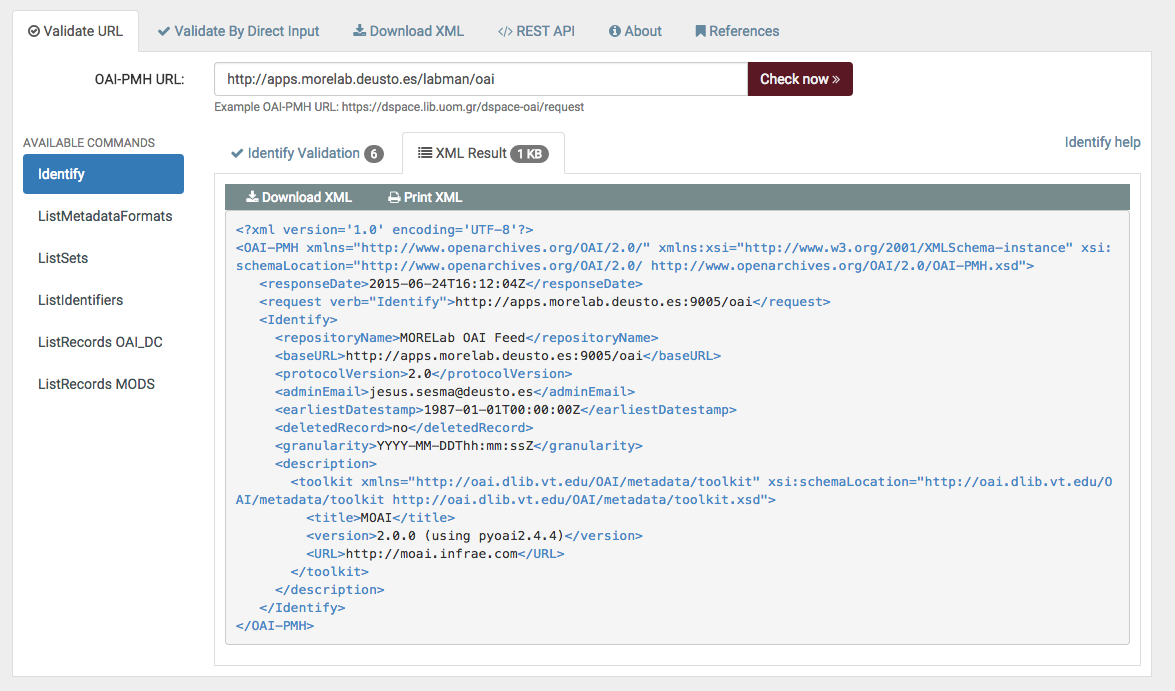
\includegraphics[scale=0.31]{fig/download_oai/download_identify}
	\caption{Información del comando Identify desde \acrshort{oaipmh} validator}
	\label{fig:download_identify}
\end{figure}

\subsection{Obtener la información del comando ListMetadataFormats}

Para descargar la información del comando ListMetadataFormats desde el propio navegador ha de realizarse una petición GET a la \acrshort{url} del servidor especificando dicho verbo mediante un \textit{query string}.

Al igual que para el comando \textit{Identify}, para descargarla desde \acrshort{oaipmh} validator es necesario introducir la \acrshort{url} del repositorio \acrshort{oai} y pulsar en el botón validate, si se introduce una \acrshort{url} de un repositorio válida aparecerán las operaciones disponibles del servidor.

Se deberá seleccionar el comando \textit{ListMetadataFormats} y escoger la pestaña \textit{\acrshort{xml} result} para acceder a la información.

\subsection{Obtener la información del comando ListSets}

Para descargar la información del comando ListSets desde el propio navegador ha de realizarse una petición GET a la \acrshort{url} del servidor especificando dicho verbo mediante un \textit{query string}.

Al igual que para el comando \textit{Identify}, para descargarla desde \acrshort{oaipmh} validator es necesario introducir la \acrshort{url} del repositorio \acrshort{oai} y pulsar en el botón validate, si se introduce una \acrshort{url} de un repositorio válida aparecerán las operaciones disponibles del servidor.

Se deberá seleccionar el comando \textit{ListSets} y escoger la pestaña \textit{\acrshort{xml} result} para acceder a la información.

\subsection{Obtener la información del comando ListIdentifiers}

Para descargar la información del comando ListSets desde el propio navegador ha de realizarse una petición GET a la \acrshort{url} del servidor especificando dicho verbo y el formato bibliográfico en el que se desea que se devuelva la consulta mediante \textit{query strings}, pudiendo filtrar por \textit{set}, \textit{from} y \textit{to}.

Esta consulta devolverá los cien primeros identificadores del repositorio, además de una clave para continuar la consulta de los siguientes cien elementos, cada vez que se quiera continuar la consulta se deberá hacer uso de dicho código, hasta que la consulta resultante disponga menos de cien recursos. 

Al igual que para el comando \textit{Identify}, para descargarla desde \acrshort{oaipmh} validator es necesario introducir la \acrshort{url} del repositorio \acrshort{oai} y pulsar en el botón validate, si se introduce una \acrshort{url} de un repositorio válida aparecerán las operaciones disponibles del servidor.

Se deberá seleccionar el comando \textit{ListSets} y escoger la pestaña \textit{\acrshort{xml} result} para acceder a la información, sin embargo la información de este comando estará limitado a los cien primero recursos del repositorio.

\subsection{Obtener la información del comando ListRecords}

Para descargar la información del comando ListRecords desde el propio navegador ha de realizarse una petición GET a la \acrshort{url} del servidor especificando dicho verbo y el formato bibliográfico en el que se desea que se devuelva la consulta mediante \textit{query strings}, puediendo filtrar por \textit{set}, \textit{from} y \textit{to}.

Esta consulta devolverá los cien primeros identificadores del repositorio, además de una clave para continuar la consulta de los siguientes cien elementos, cada vez que se quiera continuar la consulta se deberá hacer uso de dicho código, hasta que la consulta resultante disponga menos de cien recursos.

\begin{figure}[!htbp]
	\centering
	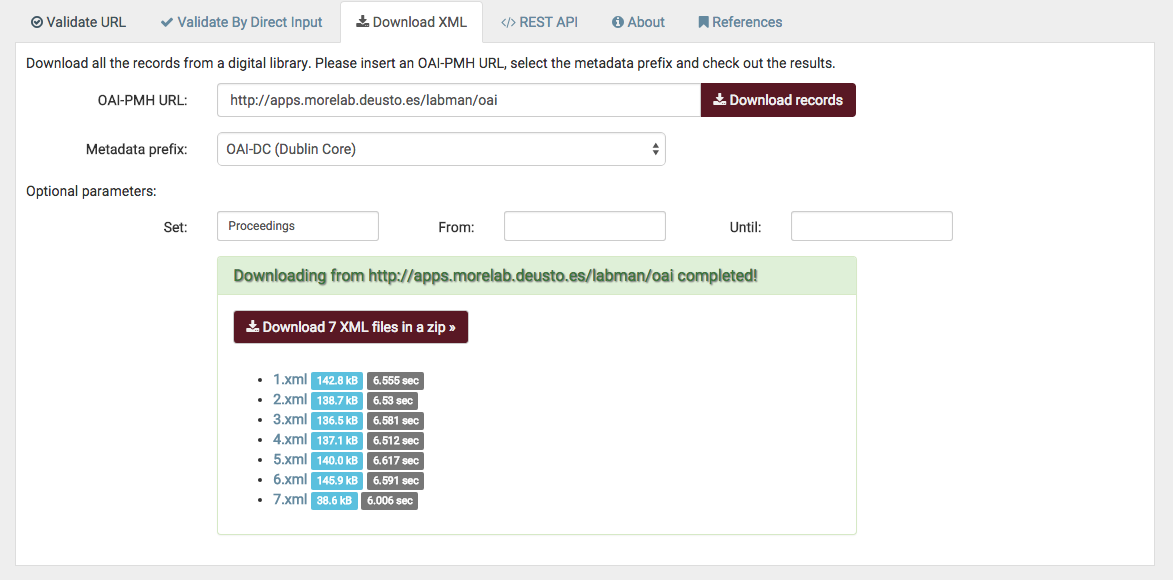
\includegraphics[scale=0.31]{fig/download_oai/download_listrecords}
	\caption{Información del comando ListRecords desde \acrshort{oaipmh} validator}
	\label{fig:download_listrecords}
\end{figure}

Para descargar la información del comando ListRecords se deberá acceder a la pestaña \textit{Download} \acrshort{xml} e introducir la \acrshort{url} del repositorio. Adicionalmente se puede filtrar los recursos por \textit{set} y por rango temporal \textit{from} y \textit{to}.

Por último se deberá pulsar en el botón \textit{Download records} para que genere los documentos \acrshort{xml}, estos se podrán descargar tanto individualmente como empaquetados en un zip tal y como se puede ver en la imagen \ref{fig:download_listrecords}.

\subsection{Obtener la información del comando GetRecord}

Para descargar la información del comando GetRecord desde el propio navegador ha de realizarse una petición GET a la \acrshort{url} del servidor especificando dicho verbo y el formato bibliográfico en el que se desea que se devuelva la consulta mediante \textit{query strings}

Para descargar la información de un recurso en concreto al igual que para \textit{ListRecords} hay que acceder a la pestaña \textit{Download} \acrshort{xml} e introducir la url del repositorio junto los \textit{query string} en la propia \acrshort{url} del repositorio para descargar la información como se muestra en la figura \ref{fig:download_getrecord}.

\begin{figure}[!htbp]
	\centering
	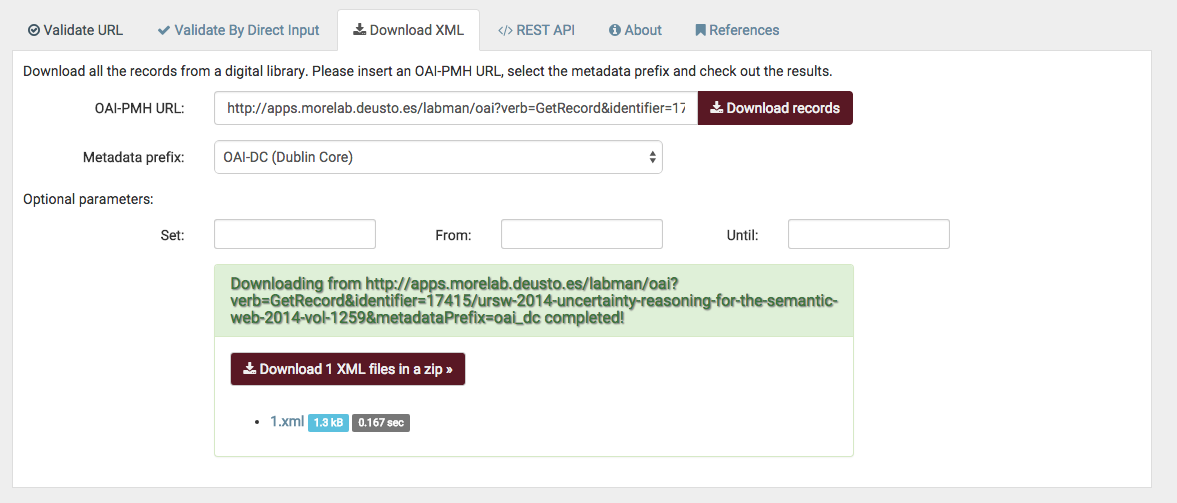
\includegraphics[scale=0.31]{fig/download_oai/download_getrecord}
	\caption{Información del comando GetRecord desde \acrshort{oaipmh} validator}
	\label{fig:download_getrecord}
\end{figure}

\section{Manual de usuario de la aplicación web}

\subsection{Página principal de LabMan}

Nada más acceder al portal web de \acrshort{labman}, se visualiza su \textit{homepage} (ver figura \ref{fig:morelab_homepage}). En ella se muestra una imagen con los miembros del grupo, la descripción y las últimas noticias relacionadas con el equipo de investigación en cuestión.

Por otra parte, se presenta una barra de navegación, con todas las siguientes opciones que ofrece \acrshort{labman} por defecto:

\begin{itemize}
	\item \textbf{News:} Muestra un buscador paginado con el registro \acrfull{rss} de las noticias relacionadas con el equipo de investigación.
	\item \textbf{Projects:} Muestra un buscador paginado con el registro de los proyectos que involucran a los miembros del equipo de investigación.
	\item \textbf{Publications:} Muestra un buscador paginado con el registro de las publicaciones redactadas por los miembros del equipo de investigación.
	\item \textbf{Member:} Muestra la lista con los integrantes del grupo de investigación.
	\item \textbf{Charts:} Muestra el menú por el que se accederán a las gráficas formadas a partir de los datos de los apartados anteriores.
	\item \textbf{About:} Muestra información adicional relacionada con el grupo de investigación.
\end{itemize}

\begin{figure}[!htbp]
	\centering
	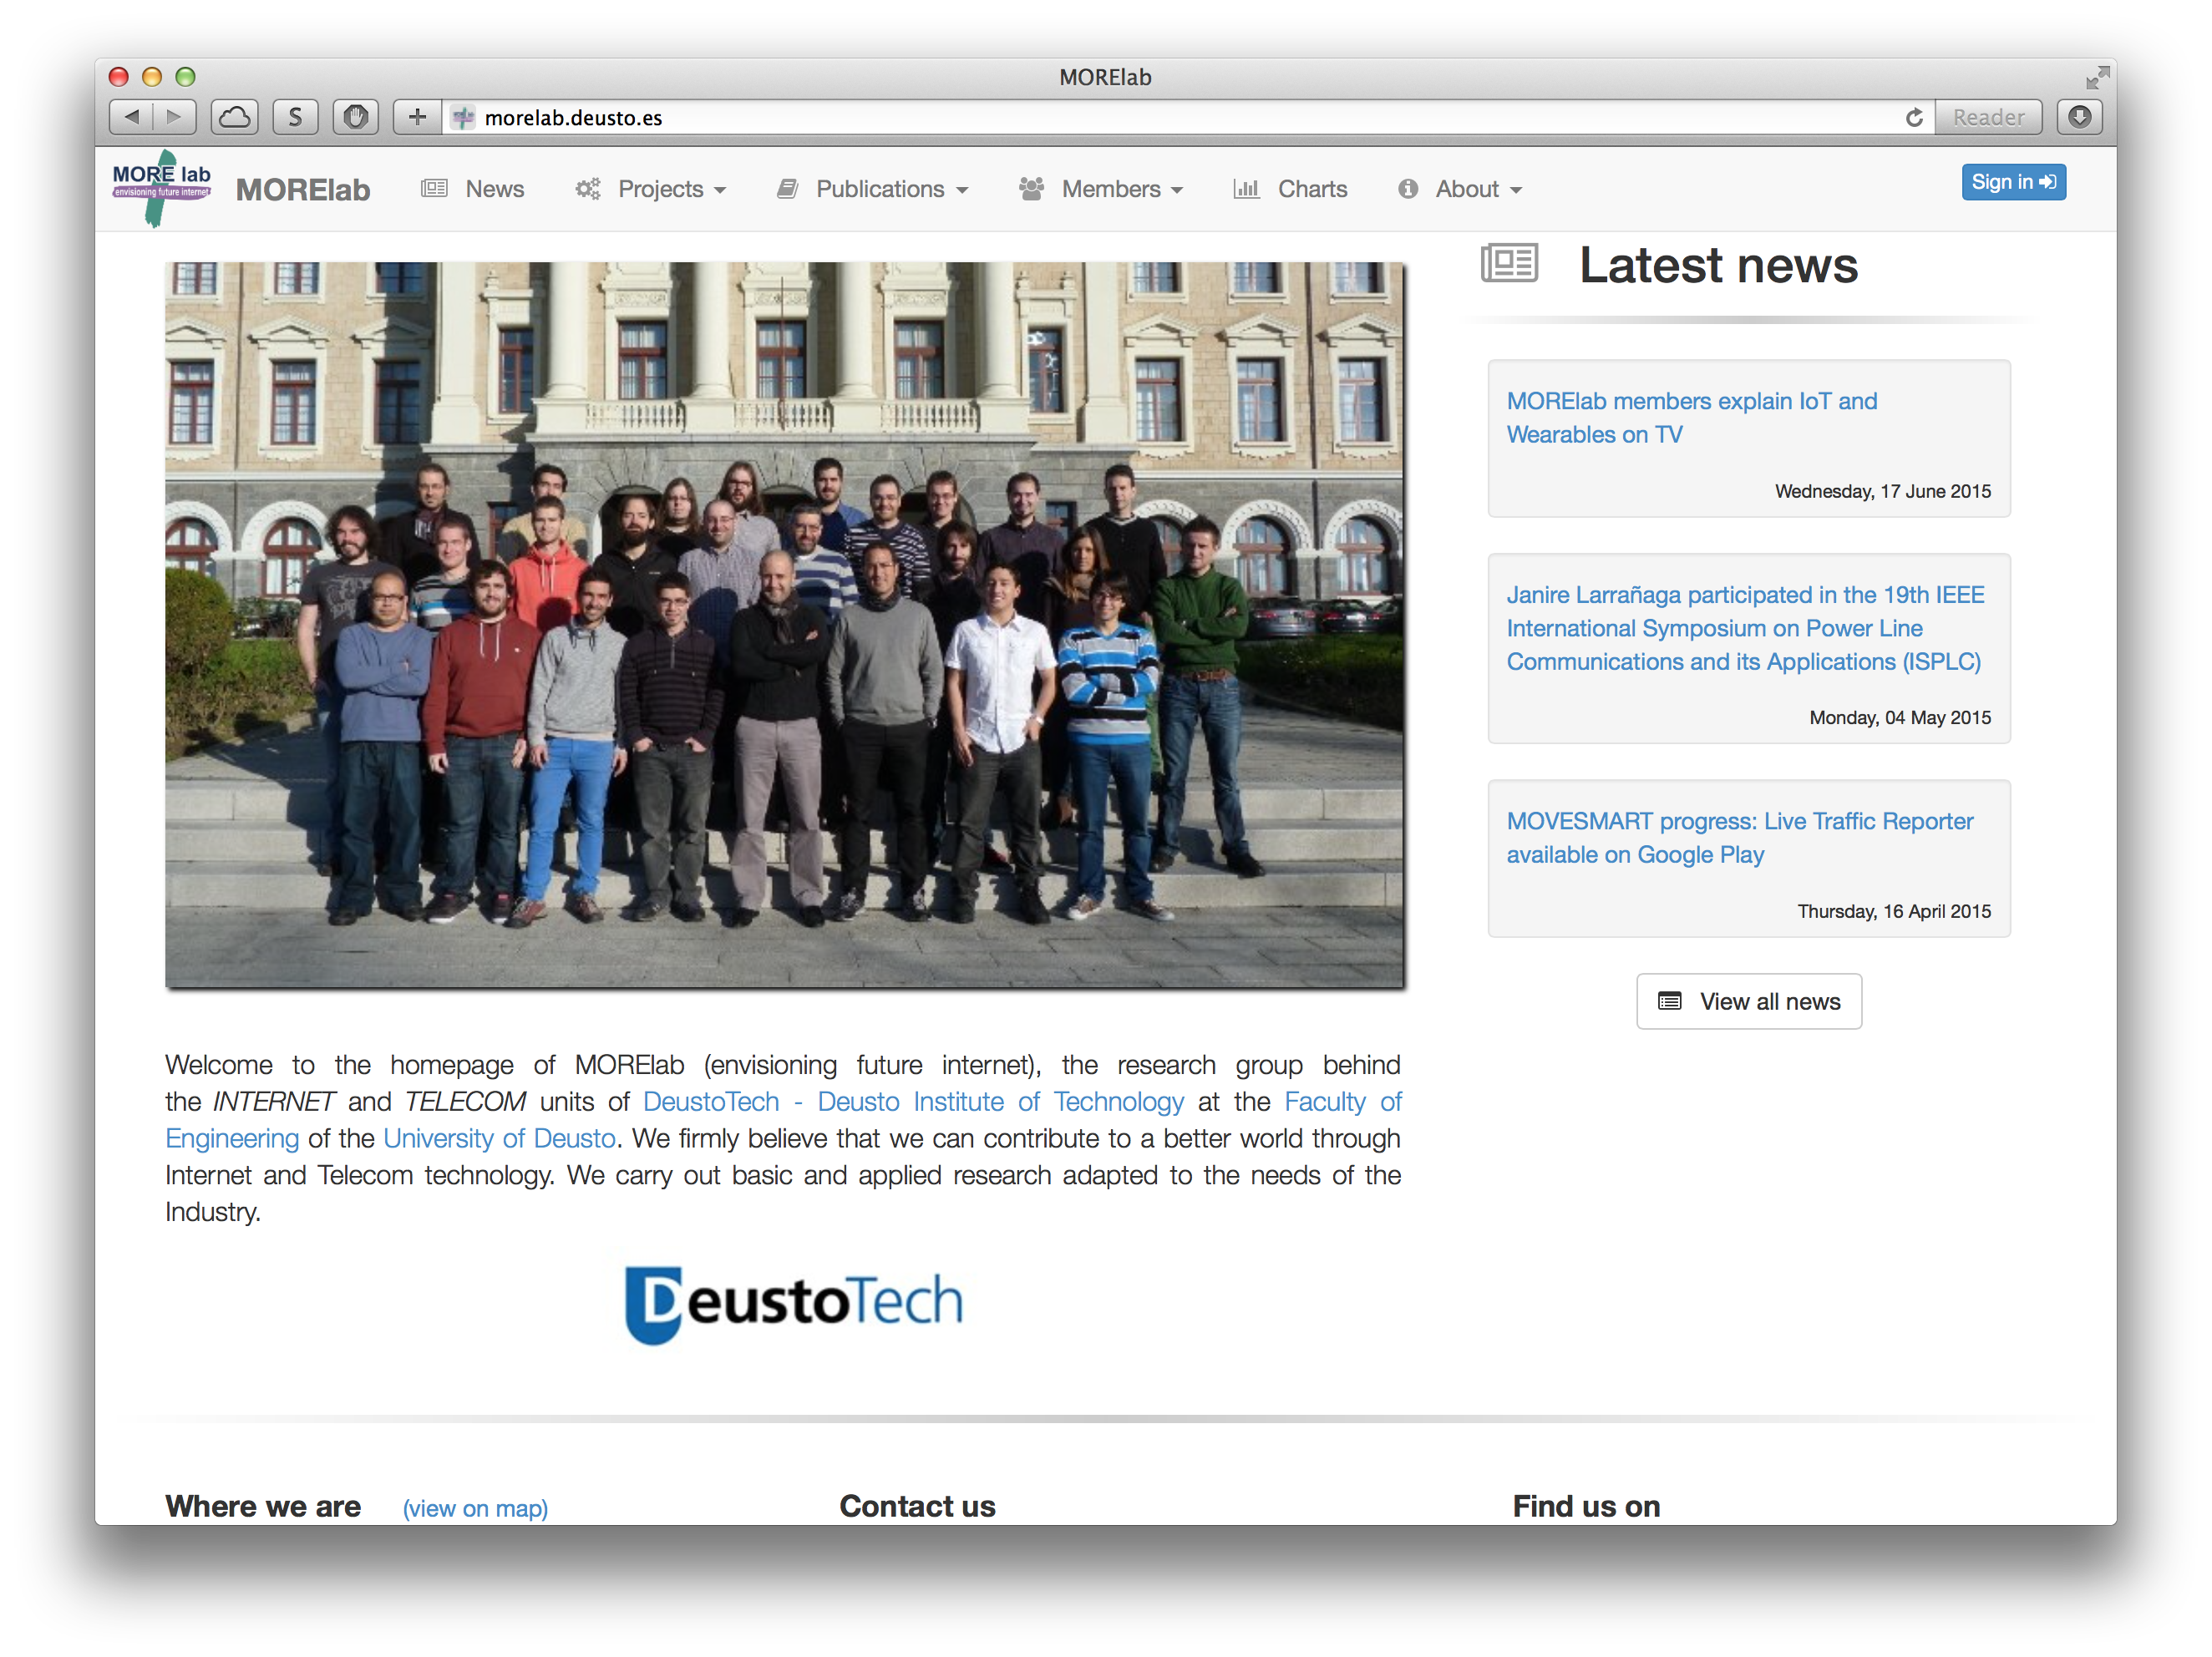
\includegraphics[scale=0.31]{fig/morelab_homepage}
	\caption{Página principal de \acrshort{labman} del equipo MoreLab}
	\label{fig:morelab_homepage}
\end{figure}

Este manual se centra en las opciones de \textit{Projects} y \textit{Publications}, dado que estas son las facetas en las que se ha trabajado a lo largo del proyecto y el resto están fuera del alcance.

\subsection{Projects: buscador de proyectos de LabMan}

Esta página muestra en principio la lista de todos los proyectos que involucran a los miembros del equipo de investigación sin filtrar. Mediante la barra de búsqueda para consultas sencillas (véase la figura \ref{fig:project_search_bar}), permite filtrar los proyectos por título o por el nombre del investigador que participe en los mismos.

\begin{figure}[!htbp]
	\centering
	
\includegraphics[scale=0.35]{fig/project_search_bar}
	\caption{Barra de búsqueda de consultas simples}
	\label{fig:project_search_bar}
\end{figure}

Sin embargo, al pulsar el botón con el símbolo \textbf{+} de la barra de búsquedas, se muestra un panel para realizar búsquedas avanzadas tal y como se muestra en la figura \ref{fig:projects_advanced_search}.

\begin{figure}[!htbp]
	\centering
	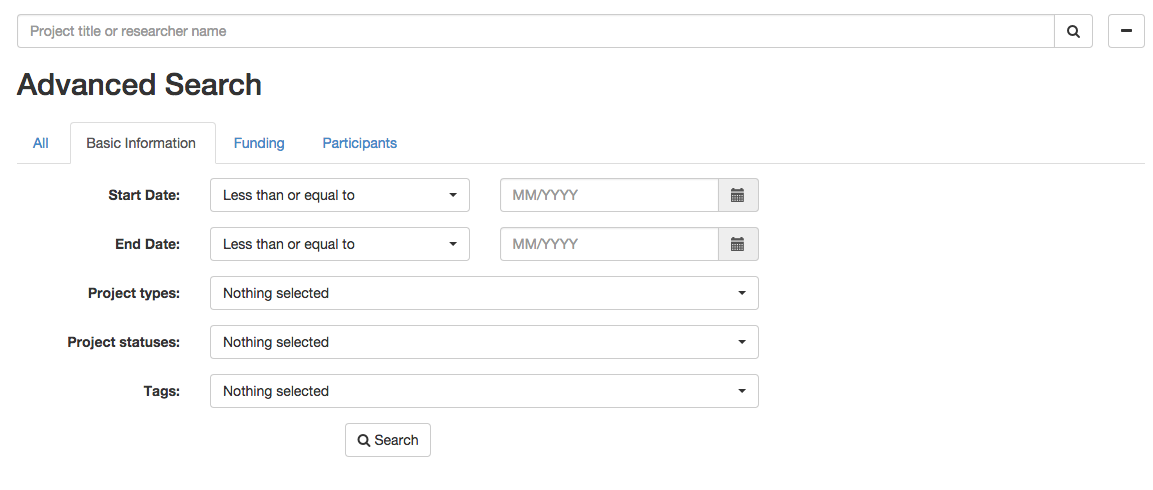
\includegraphics[scale=0.31]{fig/projects_advanced_search}
	\caption{Búsqueda avanzada de proyectos}
	\label{fig:projects_advanced_search}
\end{figure}

Mediante este buscador avanzado, se pueden filtrar los proyectos a partir de los siguientes características:

\begin{itemize}
	\item Basic information
	\begin{itemize}
		\item \textbf{Project title:} Busca todos los proyectos que contengan alguna de las palabras introducidas en este campo.
		\item \textbf{Start date:} Busca todos los proyectos que tengan una fecha de inicio menor, menor o igual, mayor, mayor o igual o igual a la introducida en este campo (formato MM/YYYY).
		\item \textbf{End date:} Busca todos los proyectos que tengan una fecha de fin menor, menor o igual, mayor, mayor o igual o igual a la introducida en este campo (formato MM/YYYY).
		\item \textbf{Project types:} Busca todos los proyectos que coincidan con alguno de los tipos de proyectos seleccionados en este campo.
		\item \textbf{Project statues:} Busca todos los proyectos que coincidan con alguno de los estados de proyectos seleccionados en este campo.
		\item \textbf{Tags:} Busca todos los proyectos que estén relacionados con alguno de las etiquetas seleccionadas en este campo.
	\end{itemize}
	\item Funding
	\begin{itemize}
		\item \textbf{Total funds:} Busca todos los proyectos cuya financiación total sea la cantidad en Euros especificada en este campo.
	\end{itemize}
	\item Participants
	\begin{itemize}
		\item \textbf{Member:} Busca todos los proyectos en los que haya participado los investigadores del grupo de investigación ejecutando alguno de los posibles roles seleccionados en este campo.
	\end{itemize}
\end{itemize}

Una vez se hayan definidos los valores de las características por las que se desea filtrar los proyectos se deberá pulsar el botón \textbf{Search} para comenzar la búsqueda y visualizar el resultado como puede mostrarse en la figura \ref{fig:projects_search_result}.

\begin{figure}[!htbp]
	\centering
	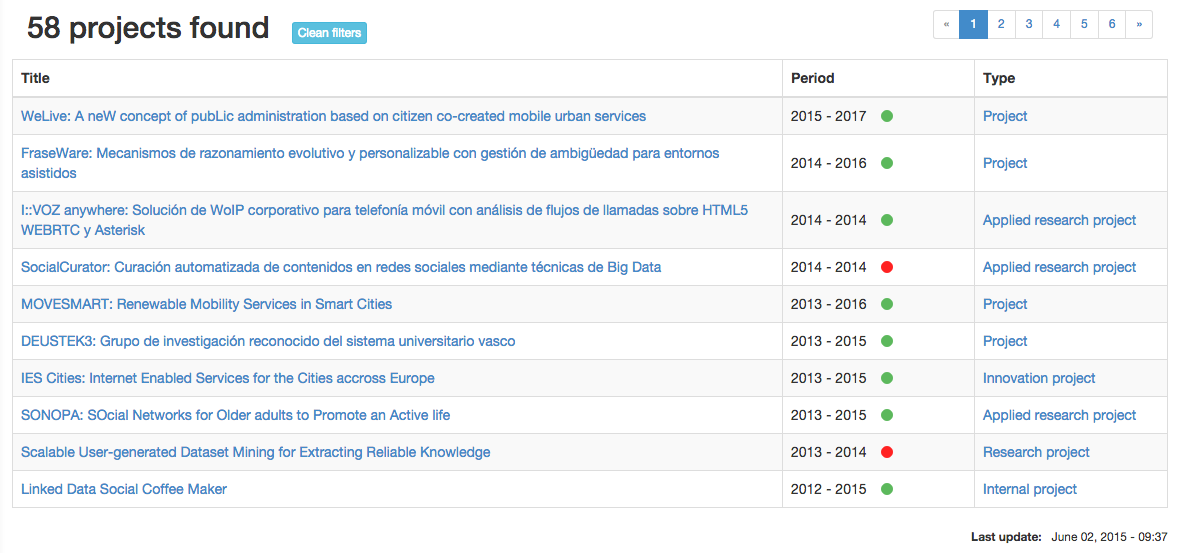
\includegraphics[scale=0.31]{fig/projects_search_result}
	\caption{Resultado de la búsqueda de proyectos}
	\label{fig:projects_search_result}
\end{figure}

\subsection{Publications: buscador de publicaciones de LabMan}

Esta página muestra en principio la lista de todos las publicaciones redactados por los miembros del equipo de investigación sin filtrar. Del mismo modo que con los proyectos, mediante la barra de búsqueda para consultas sencillas (véase la figura \ref{fig:publication_search_bar}), permite filtrar las publicaciones por título o por el nombre del investigador que ha contribuido a las mismas.

\begin{figure}[!htbp]
	\centering
	
\includegraphics[scale=0.35]{fig/publication_search_bar}
	\caption{Barra de búsqueda de consultas simples de publicaciones}
	\label{fig:publication_search_bar}
\end{figure}

Sin embargo, al pulsar el botón con el símbolo \textbf{+} de la barra de búsquedas, se muestra un panel para realizar búsquedas avanzadas tal y como se muestra en la figura \ref{fig:publications_advanced_search}.

\begin{figure}[!htbp]
	\centering
	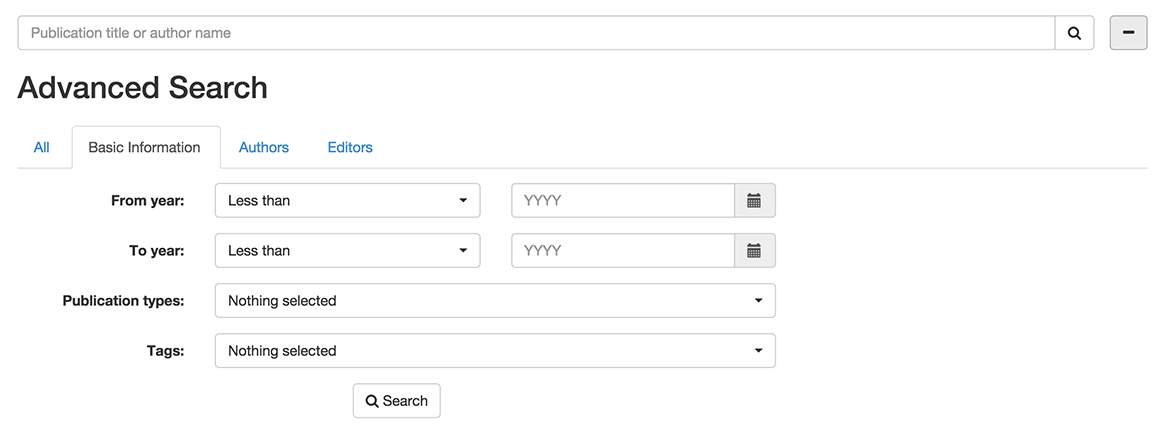
\includegraphics[scale=0.7]{fig/publications_advanced_search}
	\caption{Búsqueda avanzada de publicaciones}
	\label{fig:publications_advanced_search}
\end{figure}

Mediante este buscador avanzado, se pueden filtrar las publicaciones a partir de los siguientes características:

\begin{itemize}
	\item Basic information
	\begin{itemize}
		\item \textbf{Publication title:} Busca todos las publicaciones que contengan alguna de las palabras introducidas en este campo.
		\item \textbf{From year:} Busca todos los publicaciones que tengan un menor, menor o igual, mayor, mayor o igual o igual a la introducida en este campo (formato YYYY).
		\item \textbf{To year:} Busca todos los publicaciones que tengan un menor, menor o igual, mayor, mayor o igual o igual a la introducida en este campo (formato YYYY).
		\item \textbf{Publication types:} Busca todos las publicaciones que coincidan con alguno de los tipos de publicaciones seleccionados en este campo.
		\item \textbf{Tags:} Busca todos las publicaciones que estén relacionados con alguno de las etiquetas seleccionadas en este campo.
	\end{itemize}
	\item Authors
	\begin{itemize}
		\item \textbf{Author:} Busca todos las publicaciones que tenga a los investigadores del grupo de investigación seleccionados en este campo como autores.
	\end{itemize}
	\item Editors
	\begin{itemize}
		\item \textbf{Editor:} Busca todos las publicaciones que tenga a los investigadores del grupo de investigación seleccionados en este campo como editores.
	\end{itemize}
\end{itemize}

Una vez se hayan definidos los valores de las características por las que se desea filtrar los proyectos se deberá pulsar el botón \textbf{Search} para comenzar la búsqueda y visualizar el resultado como puede mostrarse en la figura \ref{fig:publications_search_result}.

\begin{figure}[!htbp]
	\centering
	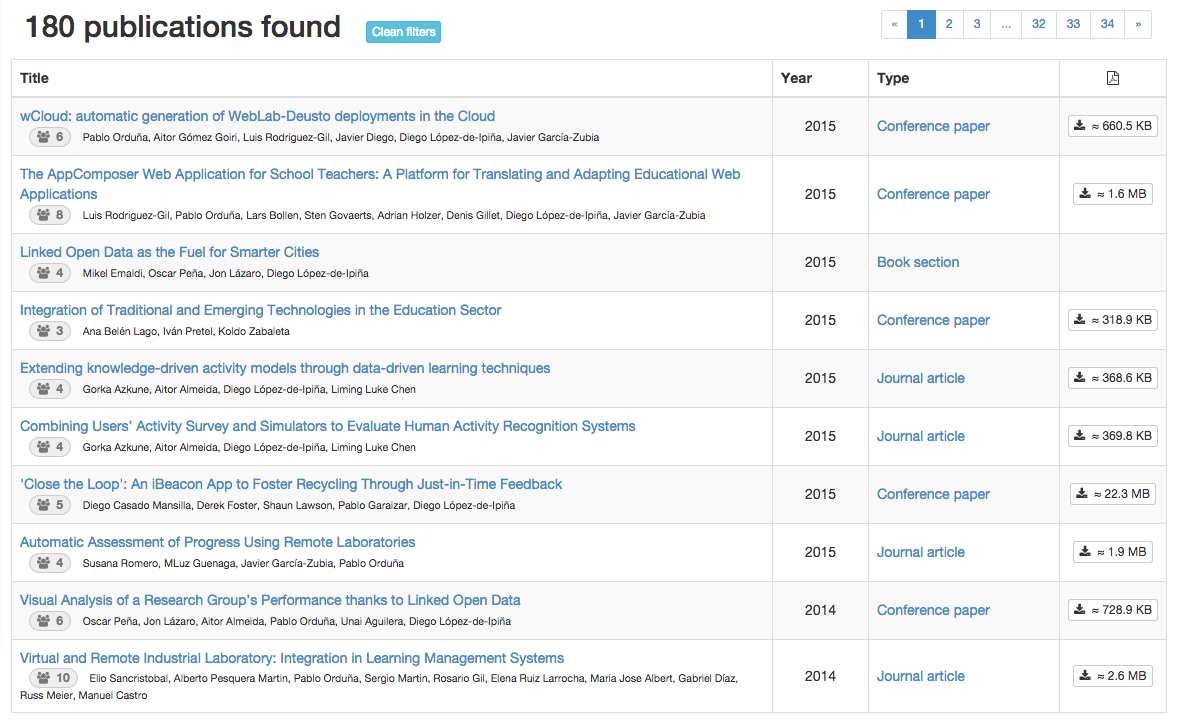
\includegraphics[scale=0.31]{fig/publications_search_result}
	\caption{Resultado de la búsqueda de publicaciones}
	\label{fig:publications_search_result}
\end{figure}
